\documentclass[../main.tex]{subfiles}

\begin{document}

\section{Cinématique}

\[
  \ac(t)=\diff{\vi}{t}=\dot{\vi}=\ddot{\pos}=
  \diff[2]{}{t}\left(x_1\vv{u}_1 + x_2\vv{u}_2 + x_3\vv{u}_3\right)
\]

\[
  \ac=\diff{v}{t}\vv{u_t} + v\diff{\vv{u_t}}{t} = \diff{v}{t}\vv{u_t} + \frac{v^2}{R_c}\vv{u_n}
\]

\subsection{Coordnonnée cylindrique}
\begin{center}
  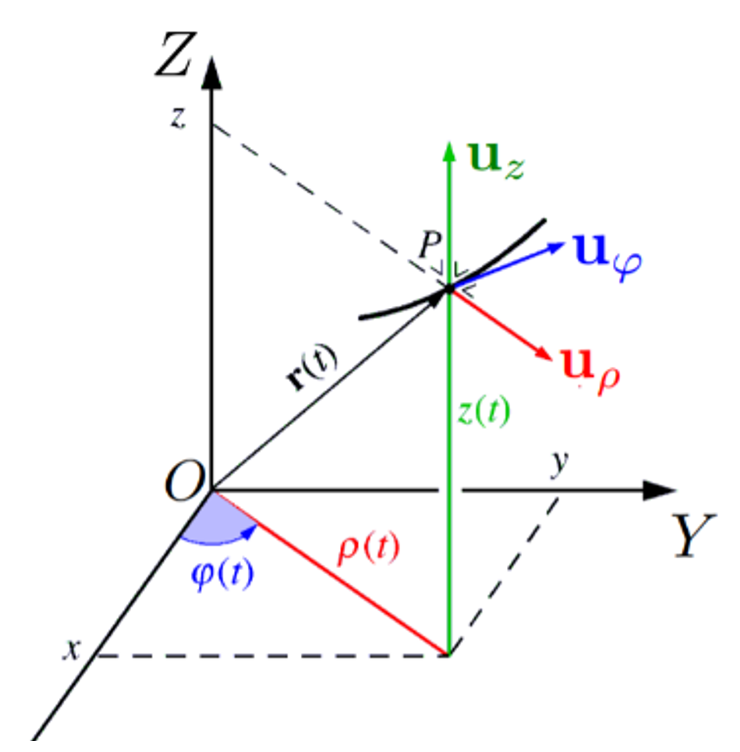
\includegraphics[width=0.1\textwidth]{images/PHYSIQUEI_1.png}
  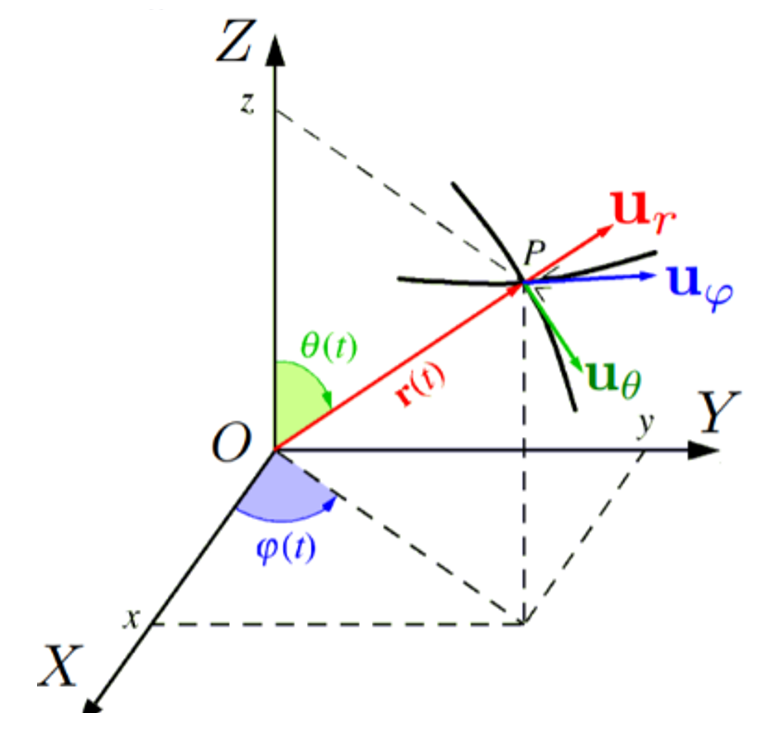
\includegraphics[width=0.1\textwidth]{images/PHYSIQUEI_2.png}
\end{center}

\vspace{-0.4cm}
\[
  \ddt\urho=\dot{\varphi}\uphi \phantom{xxx} \ddt\uphi=-\dot{\varphi}\urho
\]
\begin{IEEEeqnarray*}{rCl}
  \vi
  \begin{cases}
    v_{\rho} = \dot{\rho}\\
    v_{\varphi} = \rho\dot{\varphi}\\
    v_{z} = \dot{z}
  \end{cases}
    &
    \ac
    \begin{cases}
      a_{\rho} = \ddot{\rho} - \rho\dot{\varphi}^2\\
      a_{\varphi} = 2\dot{\rho}\dot{\varphi} + \rho\ddot{\varphi}\\
      a_{z} = \ddot{z}
    \end{cases}
\end{IEEEeqnarray*}

\subsection{Coordnonnée sphérique}
\vspace{-0.3cm}
\[
  \begin{array}{rl}
    \ddt{\ur}&=\dot{\theta}\utheta+\dot{\varphi}\sin\theta\uphi \\
    \ddt{\utheta}&=-\dot{\theta}\ur+\dot{\varphi}\cos\theta\uphi \\
    \ddt{\uphi}&=-\dot{\varphi}\sin\theta\ur-\dot{\varphi}\cos\theta\utheta\\
  \end{array}
\]
\begin{IEEEeqnarray*}{rCl}
  \vi
  \begin{cases}
    v_{r} = \dot{r}\\
    v_{\theta} = r\dot{\theta}\\
    v_{\varphi} = r\dot{\varphi}\sin{\theta}
  \end{cases}
    & \ac
    \begin{cases}
      a_{r} = \ddot{r} - r\dot{\theta}^2 - r\dot{\varphi}^2 \sin^2\theta \\
      a_{\theta} = r\ddot{\theta} + 2\dot{r}\dot{\theta} - r\dot{\varphi}^2 \cos\theta \sin\theta \\
      a_{\varphi} = r\ddot{\varphi} \sin\theta + 2r\dot{\varphi}\dot{\theta} \cos\theta + 2\dot{r}\dot{\varphi} \sin\theta
    \end{cases}
\end{IEEEeqnarray*}

\subsection{Changement de base}
Cartésien-cylindrique : 
\[
  \begin{array}{ll}
    \urho=\cos\varphi\ux + \sin\varphi\uy &
    \ux = \cos\varphi\urho - \sin\varphi\uphi\\

    \uphi=-\sin\varphi\ux + \cos\varphi\uy &
    \uy = \sin\varphi\urho + \cos\varphi\uphi\\

    \uz=\uz & \uz=\uz
  \end{array}
\]

Cartésien-sphérique : 
\begin{align*}
  \ur&=\sin\theta\cos\varphi\ux + \sin\theta\sin\varphi\uy + \cos\theta\uz\\
  \utheta&=\cos\theta\cos\varphi\ux + \cos\theta\sin\varphi\uy - \sin\theta\uz\\
  \uphi&=-\sin\varphi\ux + \cos\varphi\uy\\\\
  \ux&=\sin\theta\cos\varphi\ur + \cos\theta\cos\varphi\utheta - \sin\varphi\uphi\\
  \uy&=\sin\theta\sin\varphi\vv{u}_r + \cos\theta\sin\varphi\utheta + \cos\varphi\uphi\\
  \uz&=\cos\theta\ur - \sin\theta\utheta
\end{align*}

Cylindrique-sphérique : 
\[
  \begin{array}{ll}
    \urho = \sin\theta\ur + \cos\theta\utheta &
    \ur =\sin\theta\urho + \cos\theta\uz\\ 

    \uphi = \uphi &
    \utheta = \cos\theta\urho - \sin\theta\uz \\

    \uz = \cos\theta\ur - \sin\theta\utheta &
    \uphi = \uphi
  \end{array}
\]

\end{document}
